% Chapter 2 — Design of the ReconX framework
\chapter{Design of the ReconX Framework}
\label{chap:02}
\setlength{\parskip}{1em}

This chapter presents the design of the proposed framework. It is organized in the order in which a reader is expected to evaluate the design: first the requirements, then the high-level architecture, then each major subsystem (the finding registry, the pipeline scheduler, the scope-enforcement layer, the configuration system, the correlator, the asset-risk model, the reporting layer, and the LLM integration), and finally the deliberate limitations of the design.

\section{Functional and Non-Functional Requirements}

The framework must satisfy the following \textbf{functional} requirements (\textbf{F}):

\begin{description}[style=multiline, leftmargin=1.5cm, labelwidth=1.3cm]
  \item[F1.]  Accept a target hostname or root domain on the command line and produce a complete external-pentest report without further user interaction.
  \item[F2.]  Enumerate the public attack surface of the target: subdomains (passive and active), DNS records, live HTTP/HTTPS hosts, exposed ports and services, technology stack, CMS in use, virtual hosts, and source-map artifacts.
  \item[F3.]  Map the application surface: crawl every live host, brute-force directories, parse \texttt{robots.txt} / \texttt{sitemap.xml}, parse OpenAPI specifications, and enumerate hidden parameters.
  \item[F4.]  Audit configuration-level security properties: TLS, security headers, CORS, authentication cookies, JWT tokens, and OpenAPI security anti-patterns. Hunt for secrets in publicly served JavaScript and in associated public GitHub repositories.
  \item[F5.]  Run active probes for the OWASP Top~10 (2021) classes most relevant to external testing of a web application: reflected XSS, SQL injection, IDOR / BOLA, host header injection, web cache poisoning, server-side prototype pollution, open redirect, SSRF, SSTI, XXE, HTTP request smuggling, insecure deserialization, race conditions, GraphQL authorization gaps, OAuth misconfiguration, and WebSocket origin validation.
  \item[F6.]  Correlate findings across probes (for example, escalate the severity of a wildcard CORS finding that occurs on an authenticated endpoint) and rank assets by an aggregate risk score.
  \item[F7.]  Generate a structured HTML report for human readers, a SIEM-compatible JSON export for automated consumers, an append-only audit log of every issued HTTP request, and a Telegram notification stream for long-running scans.
  \item[F8.]  Generate a natural-language analytical report through a local LLM, with a clean fallback to an OpenAI-compatible API and a clean degradation when no LLM is available at all.
\end{description}

The framework must also satisfy the following \textbf{non-functional} requirements (\textbf{N}):

\begin{description}[style=multiline, leftmargin=1.5cm, labelwidth=1.3cm]
  \item[N1.]  \textbf{Reproducibility.} Two consecutive scans of the same target with the same configuration must produce comparable output; deltas between scans must be obtainable via a built-in diff tool.
  \item[N2.]  \textbf{Modularity.} Adding a new probe must not require changes to any existing probe; each probe is responsible for one class of analysis and communicates with the rest of the framework only through the shared finding schema.
  \item[N3.]  \textbf{Scope enforcement.} The framework must refuse to send a request to a host outside the configured scope, and this enforcement must be implemented at a layer below every probe.
  \item[N4.]  \textbf{Recoverability.} A scan must be resumable after a crash, after a network interruption, or after a deliberate \texttt{Ctrl+C} interrupt. The framework must not redo work that has already been completed.
  \item[N5.]  \textbf{Rate control.} The total request rate produced by the framework must be capped at a configurable value, both per module and globally, in order to avoid disrupting the target.
  \item[N6.]  \textbf{Triage clarity.} Every finding must carry a \textit{verdict} that distinguishes \textit{confirmed} weaknesses from \textit{candidate} weaknesses that still require manual review.
  \item[N7.]  \textbf{No commercial licenses.} The framework must run on a standard Kali-Linux workstation without paid subscriptions; integrations with paid services are optional.
\end{description}

\section{High-Level Architecture}

Figure~\ref{fig:arch} summarizes the architecture of the framework. The framework is implemented in pure Python~3 as a set of cooperating modules organized into four logical layers:

\begin{enumerate}
  \item the \textbf{pipeline orchestrator} (the \texttt{main.py} entry point) that reads command-line arguments and configuration, loads the modules of the pipeline, and schedules their execution;
  \item a \textbf{module layer} consisting of 46 specialized Python classes, each one a subclass of \texttt{BaseModule} (passive) or \texttt{ActiveProbeBase} (active), and each one responsible for a single class of analysis;
  \item a \textbf{cross-cutting services layer} that provides the finding registry, the rate limiter, the audit logger, the scope enforcer, the resume cache, the AI advisor, and the Telegram notifier;
  \item a \textbf{reporting layer} that consumes the unified finding stream and produces \texttt{report.html}, \texttt{report.json}, \texttt{audit.jsonl}, and the post-scan AI analysis.
\end{enumerate}

\begin{figure}[H]
\centering
\fbox{\begin{minipage}{0.92\textwidth}
\small
\texttt{[CLI args]} $\rightarrow$ \texttt{main.py} $\rightarrow$ \textbf{Pipeline orchestrator}\\[1mm]
\hspace*{0.5cm}$\downarrow$ load + apply preset $\downarrow$\\[1mm]
\texttt{config.yaml} $\rightarrow$ \textbf{Configuration} $\leftrightarrow$ \textbf{Scope enforcer}\\[1mm]
\hspace*{0.5cm}$\downarrow$ schedule modules by group $\downarrow$\\[1mm]
\textbf{Group 1--5: Reconnaissance} (recon, secret\_scanner, portscan, webdetect, techstack, spa\_crawler, fuzzer, ssl\_checker, cors\_checker, auth\_probe, cmscan, sourcemap\_analyzer, vhost\_enum, takeover\_checker, openapi\_parser)\\[1mm]
\textbf{Group 6: Discovery} (parameter\_discovery)\\[1mm]
\textbf{Group 7--9: Probes} (http\_smuggling, jwt\_audit, websocket\_probe, api\_schema\_audit, js\_security\_audit, oauth\_probe, cache\_poison, host\_header\_injection, open\_redirect\_probe, prototype\_pollution, deserialization\_probe, race\_condition, graphql\_audit, api\_key\_validator, xxe\_probe)\\[1mm]
\textbf{Group 10: Heavy injection} (xss, sql\_injection, idor\_probe, injection\_probe)\\[1mm]
\textbf{Group 11: Nuclei} (vulnscan)\\[1mm]
\textbf{Group 12--14: Post-processing} (cve\_check, correlator, asset\_risk)\\[1mm]
\textbf{Group 15: AI report} (ai\_report)\\[1mm]
\hspace*{0.5cm}$\downarrow$ unified findings $\downarrow$\\[1mm]
\textbf{Finding registry} $\rightarrow$ \textbf{Reporting layer} $\rightarrow$ \texttt{report.html} / \texttt{report.json} / \texttt{audit.jsonl} / Telegram
\end{minipage}}
\caption{High-level architecture of the ReconX framework.}
\label{fig:arch}
\end{figure}

The architecture has three properties that the rest of the chapter will explore in detail. First, the modules are arranged into 15 \textit{execution groups} so that modules with no data dependency on each other can run in parallel, while modules that depend on each other are placed in successive groups. Second, every probe inherits from a small base class hierarchy that provides the cross-cutting services (scope enforcement, rate limiting, audit logging), so that the probe author never writes that code by hand. Third, every probe expresses its output through a single \texttt{build\_finding(...)} call into the finding registry, which makes every probe pluggable from the reporting layer's point of view.

\section{The Module Layer and the Pipeline Scheduler}
\label{sec:pipeline}

\subsection{The Module Contract}

Every module in the framework is a Python class that inherits from \texttt{BaseModule} (or from its active-probe subclass \texttt{ActiveProbeBase}) and exposes the methods listed in Table~\ref{tab:module-contract}.

\begin{table}[h]
\centering
\small
\begin{tabular}{|p{4.2cm}|p{8.8cm}|}
\hline
\textbf{Method / attribute} & \textbf{Role} \\
\hline
\texttt{name}, \texttt{description} & Short stable identifier and one-line description used by the orchestrator and the report renderer. \\
\texttt{required\_tools} & List of external command-line tools that the module wraps. Missing tools cause the module to skip gracefully, not to crash. \\
\texttt{run()} & Main entry point. Returns a Python dictionary that contains, at minimum, a \texttt{findings} list and any module-specific data the report renderer should display. \\
\texttt{has\_tool(name)} & Inherited helper that checks tool availability against an extended \texttt{PATH}. \\
\texttt{exec(cmd, timeout=...)} & Inherited subprocess wrapper that records the command, enforces a timeout, and respects the global Ctrl+C handler. \\
\texttt{save\_json}, \texttt{save\_text}, \texttt{load\_json} & Inherited helpers that persist intermediate artifacts inside the per-module output directory. \\
\texttt{module\_config()} (active probes) & Inherited helper that returns the module-specific configuration block from \texttt{config.yaml}, with defaults applied. \\
\texttt{make\_finding(...)} (active probes) & Inherited helper that calls \texttt{build\_finding(...)} on the finding registry and applies severity normalization, deduplication, and verdict assignment. \\
\hline
\end{tabular}
\caption{Module contract enforced by \texttt{BaseModule}.}
\label{tab:module-contract}
\end{table}

This contract is deliberately small. A new module is implemented by writing a single Python class with a single \texttt{run()} method; the rest of the framework picks it up automatically through the \texttt{PIPELINE} and \texttt{CLASS\_MAP} tables in \texttt{main.py}.

\subsection{The Pipeline and Its Execution Groups}

The orchestrator schedules the modules into 15 numbered groups (Table~\ref{tab:pipeline-groups}). Modules within a group are launched concurrently in a \texttt{ThreadPoolExecutor}; groups are executed strictly in order. After every group completes, the orchestrator persists an \texttt{all\_results.json} snapshot of every module's output so far. This snapshot is the basis of the resume mechanism described in Section~\ref{sec:resume}.

\begin{table}[h]
\centering
\small
\begin{tabular}{|c|p{4cm}|p{7cm}|}
\hline
\textbf{Group} & \textbf{Purpose} & \textbf{Modules} \\
\hline
1  & Initial reconnaissance     & recon, secret\_scanner \\
2  & Network surface            & portscan, webdetect \\
3  & Technology fingerprinting  & techstack, spa\_crawler \\
4  & Surface and configuration  & fuzzer, ssl\_checker, cors\_checker, auth\_probe \\
5  & CMS and OSINT enrichment   & cmscan, sourcemap\_analyzer, vhost\_enum, takeover\_checker, openapi\_parser \\
6  & Parameter discovery        & parameter\_discovery \\
7  & Low-traffic probes         & http\_smuggling, jwt\_audit, websocket\_probe, api\_schema\_audit, js\_security\_audit \\
8  & Medium-traffic probes      & oauth\_probe, cache\_poison, host\_header\_injection, open\_redirect\_probe, prototype\_pollution, deserialization\_probe, race\_condition, graphql\_audit \\
9  & Remaining validators       & api\_key\_validator, xxe\_probe \\
10 & Heavy injection            & injection\_probe, xss, sql\_injection, idor\_probe \\
11 & Template-based scan        & vulnscan (Nuclei) \\
12 & Component CVE lookup       & cve\_check \\
13 & Cross-finding correlation  & correlator \\
14 & Per-asset risk ranking     & asset\_risk \\
15 & AI analysis                & ai\_report \\
\hline
\end{tabular}
\caption{Pipeline groups and the modules they contain.}
\label{tab:pipeline-groups}
\end{table}

The grouping is not arbitrary. Several rules are encoded in it:

\begin{itemize}
  \item Modules that produce data consumed by later modules go first: \texttt{recon} produces the live-host list consumed by \texttt{portscan}, \texttt{webdetect}, \texttt{techstack}, and every active probe; \texttt{fuzzer} produces the endpoint catalogue consumed by \texttt{parameter\_discovery}, which in turn produces the parameter catalogue consumed by the active probes in group~10.
  \item Probes that would interfere with each other are not co-scheduled: \texttt{vulnscan} (Nuclei) is alone in group~11, because Nuclei's rate-limited runs are sensitive to the request storm that \texttt{sqlmap} produces.
  \item Post-processing modules (correlator, asset\_risk, ai\_report) are last, because they read the entire \texttt{all\_results} dictionary, not just the output of one earlier module.
\end{itemize}

\subsection{Recovery, Resume, and Per-Module Caching}
\label{sec:resume}

Every module persists its result to \texttt{output/<session>/<module>/results.json}. The orchestrator additionally persists \texttt{all\_results.json} after every group. On a subsequent invocation, the orchestrator inspects the output directory: if a module's \texttt{results.json} is already present and the input it depends on has not changed, the module's \texttt{run()} method is skipped and its cached result is loaded directly. This makes the pipeline naturally idempotent and gives the operator the freedom to re-run a single problematic module (\texttt{-m vulnscan}) without having to start over.

In addition to per-module caching, the framework keeps the last~10 snapshots of \texttt{all\_results.json} for each target in \texttt{\textasciitilde/.reconx/snapshots/<target>/}, so that a \texttt{--diff} re-run can show \textit{new} and \textit{removed} findings relative to a previous engagement.

\section{The Finding Registry}
\label{sec:registry}

The finding registry is the central design element of the framework. Every probe produces findings through a single function, \texttt{build\_finding(\dots)}, which guarantees that every finding produced by any module carries the schema shown in Table~\ref{tab:finding-schema}.

\begin{table}[h]
\centering
\small
\begin{tabular}{|l|p{10cm}|}
\hline
\textbf{Field} & \textbf{Meaning} \\
\hline
\texttt{source}       & Name of the module that emitted the finding (\texttt{xss}, \texttt{idor\_probe}, \dots). \\
\texttt{id}           & Stable, registry-defined identifier for the finding type (e.g.\ \texttt{xss\_reflected\_marker}, \texttt{cors\_wildcard\_origin}). \\
\texttt{title}        & Human-readable title, derived from the registry. \\
\texttt{severity}     & \texttt{CRITICAL}, \texttt{HIGH}, \texttt{MEDIUM}, \texttt{LOW}, or \texttt{INFO}, normalized by the registry. \\
\texttt{confidence}   & Floating-point score in $[0, 1]$ reflecting how sure the probe is that the issue is real. \\
\texttt{exploitability} & \texttt{passive}, \texttt{candidate}, \texttt{requires\_auth}, \texttt{active}, or \texttt{confirmed}. \\
\texttt{verdict}      & \texttt{confirmed}, \texttt{candidate}, or \texttt{manual\_review}, derived from severity / confidence / exploitability. \\
\texttt{cwe}          & CWE identifier looked up from the registry (e.g.\ CWE-79 for reflected XSS). \\
\texttt{cvss}         & CVSS v3.1 vector / score, when applicable. \\
\texttt{owasp}        & OWASP Top~10 category (e.g.\ \texttt{A03:2021}). \\
\texttt{attack\_technique} & MITRE ATT\&CK tactic / technique identifier (e.g.\ T1190). \\
\texttt{url}, \texttt{param} & The affected URL and request parameter, when applicable. \\
\texttt{evidence}     & Probe-specific dictionary (matched pattern, request, response excerpt, payload, marker, \dots). \\
\texttt{references}   & List of authoritative references (OWASP cheat-sheet URL, PortSwigger article, RFC). \\
\hline
\end{tabular}
\caption{Unified schema produced by the finding registry.}
\label{tab:finding-schema}
\end{table}

The registry also defines two scoring tables that are reused throughout the pipeline:

\begin{itemize}
  \item \textit{Severity weights} --- \texttt{INFO}=5, \texttt{LOW}=20, \texttt{MEDIUM}=45, \texttt{HIGH}=70, \texttt{CRITICAL}=90.
  \item \textit{Exploitability weights} --- \texttt{passive}=0.20, \texttt{candidate}=0.35, \texttt{requires\_auth}=0.50, \texttt{active}=0.65, \texttt{confirmed}=0.90.
\end{itemize}

The risk score of a single finding is the product of the severity weight, the confidence, and the exploitability weight. The asset-risk module aggregates these per-finding scores into a per-host score, and the correlator can additionally promote a finding's severity when a cross-probe rule fires.

The verdict labelling is deliberately conservative. A finding is reported as \texttt{confirmed} only when the probe has a concrete, machine-verifiable signal (marker reflected, redirect observed, parsing error returned, profile comparison detected). Anything weaker is reported as \texttt{candidate}, and weaker still as \texttt{manual\_review}. This three-way split is what allows the operator to read a long report without losing trust in the high-priority findings.

\section{Scope Enforcement, Rate Limiting, and Auditing}

These three cross-cutting concerns are implemented in \texttt{BaseModule} so that no probe can violate them by accident.

\subsection{Scope Enforcement}

The configuration accepts a \texttt{scope} block with three lists: \texttt{allowed\_domains}, \texttt{allowed\_ips}, and \texttt{excluded}. Whenever a module calls the inherited \texttt{http\_request(\dots)} helper, the helper extracts the host from the URL and checks it against the three lists. If the host is not allowed, the helper short-circuits the call, records the attempt in the audit log, and returns a \texttt{None} response to the caller. The probe's logic typically already treats \texttt{None} as a benign error, so out-of-scope requests are not just blocked but also do not produce false findings.

For probes that invoke external subprocess tools (sqlmap, Nuclei, dalfox), scope enforcement is provided in a complementary way: the orchestrator pre-filters the URL list that is passed to the tool as a command-line argument, and the tool itself runs without an internal scope concept. This is sufficient because the tools accept an explicit URL list rather than discovering new hosts on their own.

\subsection{Rate Limiting}

Each module owns a \texttt{TokenBucket} sized by its module-specific \texttt{rate\_limit} setting, and the entire process owns a single shared \texttt{TokenBucket} sized by the global \texttt{global\_rate\_limit} setting. The \texttt{http\_request(\dots)} helper acquires a token from the global bucket first and then from the module bucket, blocking the calling thread when no token is available. This guarantees that the total request rate of the process never exceeds the global limit, even when many modules run in parallel.

\subsection{Audit Logging}

Every issued HTTP request is appended as a single JSON line to \texttt{audit.jsonl} in the session output directory. Each entry records the module name, the URL, the HTTP method, the response status, the elapsed time in milliseconds, the in-scope flag, and any error reason. The audit log is append-only and write-locked per file path, so it survives crashes and concurrent writes.

\section{The Configuration System and Scan Profiles}

The framework is configured through a YAML file (\texttt{config.yaml}) that contains nine top-level sections: \texttt{api\_keys}, \texttt{auth\_profiles}, \texttt{telegram}, \texttt{ai}, \texttt{scan} (including per-module sub-blocks), \texttt{scope}, \texttt{custom\_presets}, \texttt{legal\_acknowledgment}, and \texttt{reporting}. Environment variables can override specific keys; the framework maintains a documented map of environment-variable to configuration-key bindings (for example, \texttt{OPENAI\_API\_KEY} maps to \texttt{ai.openai\_api\_key}) so that the operator never has to write a secret into the YAML file.

The configuration system additionally defines four built-in \textbf{scan profiles}, summarized in Table~\ref{tab:profiles}. A profile is a set of overrides that the orchestrator applies on top of the YAML configuration, so that the operator can change the intrusiveness of the scan with a single command-line flag.

\begin{table}[h]
\centering
\small
\begin{tabular}{|l|p{10cm}|}
\hline
\textbf{Profile} & \textbf{Effect} \\
\hline
\texttt{safe}       & Read-only operations only. Disables IDOR cross-profile comparison, disables active race-condition probing, disables prototype-pollution body probing, disables API-key live validation. \texttt{allow\_write} is forced to \texttt{false}. \\
\texttt{bug\_bounty}& Same as \texttt{safe} but with higher target counts per probe; intended for a long unattended scan over a wide bug-bounty scope. \\
\texttt{deep}       & Enables IDOR cross-profile comparison, enables active race-condition probing, enables OOB XXE confirmation when an interactsh server is available, raises sqlmap target count. Still \texttt{allow\_write=false} for the default install. \\
\texttt{intrusive}  & Enables every probe at its most aggressive configuration. Requires explicit \texttt{--legal-acknowledgment} on the command line. \\
\hline
\end{tabular}
\caption{Built-in scan profiles.}
\label{tab:profiles}
\end{table}

The combination of YAML configuration, environment-variable overrides, command-line arguments, and scan profiles is designed so that the operator can keep a single \texttt{config.yaml} and switch from a safe scope-wide bug-bounty scan to a deep authenticated test of a single application with one CLI flag.

\section{The Correlator and the Asset-Risk Module}

The correlator (\texttt{correlator.py}) and the asset-risk module (\texttt{asset\_risk.py}) operate on the assembled \texttt{all\_results} dictionary after every probe has finished. Their role is to convert a flat list of independent findings into a prioritized, asset-centric view.

\subsection{The Correlator}

The correlator evaluates a fixed set of cross-finding rules, each of which fires when a specific combination of probes has produced their respective findings. Representative rules are listed in Table~\ref{tab:correlation-rules}.

\begin{table}[h]
\centering
\small
\begin{tabular}{|p{4.8cm}|p{8.2cm}|}
\hline
\textbf{Rule} & \textbf{Condition / effect} \\
\hline
\texttt{admin\_port\_no\_waf\_cve} & Admin port reachable (\texttt{portscan}) \texttt{AND} component has known CVE (\texttt{cve\_check}) \texttt{AND} no WAF detected. \textbf{Effect:} promote to CRITICAL. \\
\texttt{public\_cloud\_storage} & S3 / GCS / Azure bucket listed publicly (\texttt{fuzzer}). \textbf{Effect:} HIGH, add data-leak tag. \\
\texttt{graphql\_mutations\_auth} & GraphQL endpoint allows mutations anonymously (\texttt{graphql\_audit}). \textbf{Effect:} HIGH. \\
\texttt{email\_spoofing} & SPF / DKIM / DMARC missing or misconfigured (\texttt{recon}). \textbf{Effect:} MEDIUM. \\
\texttt{exposed\_datastore} & Redis / MongoDB port open (\texttt{portscan}) \texttt{AND} no auth required. \textbf{Effect:} CRITICAL. \\
\texttt{docker\_api\_exposed} & Docker daemon port 2375 reachable with successful API ping. \textbf{Effect:} CRITICAL. \\
\texttt{high\_confidence\_takeover} & Dangling CNAME (\texttt{takeover\_checker}) \texttt{AND} live HTTP on host. \textbf{Effect:} HIGH. \\
\texttt{cors\_with\_auth} & Wildcard / reflected CORS \texttt{AND} \texttt{Allow-Credentials: true} on auth endpoint. \textbf{Effect:} HIGH. \\
\texttt{xss\_with\_auth} & Reflected XSS on a URL that requires an authenticated session. \textbf{Effect:} HIGH. \\
\hline
\end{tabular}
\caption{Representative correlation rules.}
\label{tab:correlation-rules}
\end{table}

The correlator emits a new synthetic finding for every rule that fires, with its own evidence pointing at the contributing probes. The synthetic finding is added to the unified finding stream, so it is rendered by the report renderer like any other finding.

\subsection{The Asset-Risk Module}

The asset-risk module groups every finding by its asset (a normalized host or URL prefix) and computes a per-asset score from the weighted contributions of the findings that target it. The weights used are:

\[
\textit{score}(asset) = \sum_{f \in F(asset)} w_{\textit{sev}(f)} \cdot c(f) \cdot w_{\textit{exp}(f)} + \textit{bonus}(asset)
\]

where $F(asset)$ is the set of findings on the asset, $w_{\textit{sev}}$ and $w_{\textit{exp}}$ are the severity and exploitability weights from Section~\ref{sec:registry}, $c(f)$ is the confidence, and $\textit{bonus}(asset)$ adds discrete contributions for context flags (exposed admin: +12; sensitive file present: +8; CVE hit: +7; takeover signal: +30). Assets are then bucketed into four tiers:

\[
\textit{tier}(s) =
\begin{cases}
\textit{critical}, & s \ge 80 \\
\textit{high},     & 50 \le s < 80 \\
\textit{medium},   & 25 \le s < 50 \\
\textit{low},      & s < 25.
\end{cases}
\]

The report renders the top 200 assets sorted by descending score, with the tier shown as a colored badge.

\section{Reporting Layer}

\subsection{HTML Report}

The HTML report is rendered from a Jinja2 template (\texttt{templates/report.html}). Static assets are embedded inline so that the report is a single self-contained file that can be sent as an email attachment. The template receives the entire \texttt{all\_results} dictionary plus the LLM analysis and renders, in order: an executive summary; the LLM analysis (Markdown-to-HTML, sanitized through Bleach); the asset-risk table; the correlator's synthetic findings; per-module sections (one per probe); and finally an appendix that lists every issued HTTP request from the audit log.

\subsection{SIEM-Compatible JSON}

The SIEM-compatible JSON export (\texttt{report.json}) flattens the unified finding stream into a list that downstream consumers can ingest with a single deserialization. Each entry carries every field from Table~\ref{tab:finding-schema}, plus the originating module, plus the asset, plus the scan metadata (start time, end time, host running the scan, framework version). The \texttt{--diff} subcommand additionally produces \texttt{diff\_results.json}, in which findings are tagged as \textit{new}, \textit{removed}, or \textit{changed} relative to the previous snapshot.

\subsection{Audit Log and Telegram Notifications}

The audit log (\texttt{audit.jsonl}) is described in the previous section. The Telegram notifier (\texttt{reporting/telegram.py}) emits five categories of message: start, periodic progress, per-module completion (with a one-line summary), error, critical-finding alert, and complete. Messages are truncated to fit Telegram's 4096-byte limit, and the notifier degrades gracefully when no \texttt{bot\_token} is configured. Figure~\ref{fig:telegram} shows a complete pair of \textit{start} and \textit{complete} messages received during the \texttt{miras.app} scan; the messages are emitted in the operator's configured locale (Russian, in this example) and the final message includes an aggregate \textit{security grade} computed from the asset-risk ranking.

\begin{figure}[H]
\centering
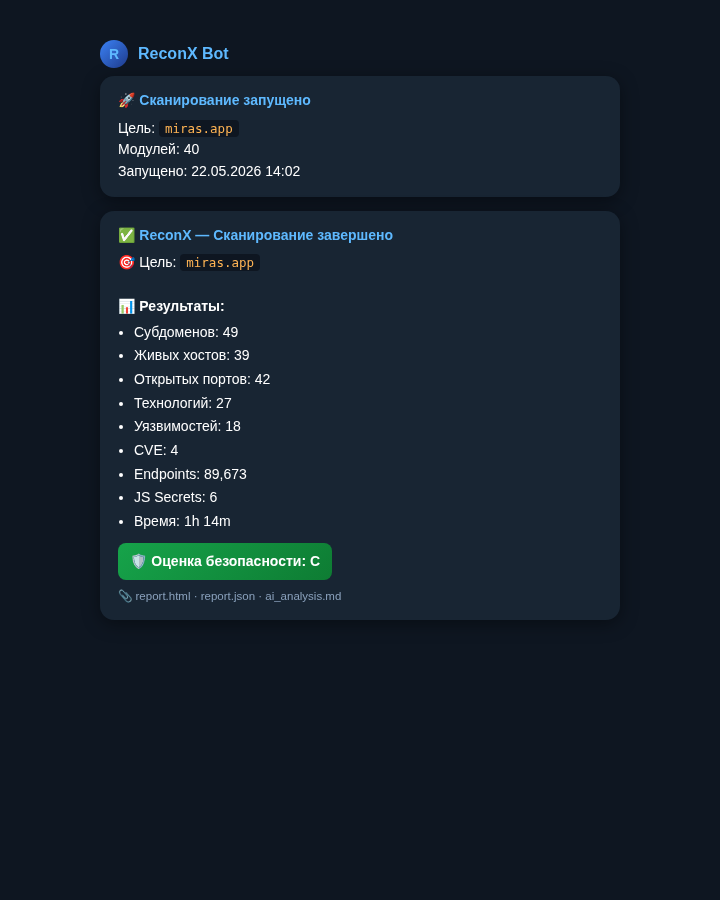
\includegraphics[width=0.55\textwidth]{images/04_telegram_summary.png}
\caption{Telegram start / complete notifications emitted during the \texttt{miras.app} scan (operator's locale: Russian).}
\label{fig:telegram}
\end{figure}

\section{The LLM Integration Layer}

The framework integrates a Large Language Model in two places: an optional real-time advisor that runs after each major probe completes, and a mandatory post-scan report module that runs as the last group of the pipeline.

\subsection{Provider Abstraction}

The integration is abstracted around two providers:

\begin{itemize}
  \item \textbf{Ollama} --- the default. Ollama is a local LLM runtime that exposes an HTTP API on \texttt{localhost:11434}. The framework sends a JSON prompt and reads back a streamed response. The default model is \texttt{deepseek-r1:7b}; the operator can switch to \texttt{qwen2.5:7b} or \texttt{llama3:8b} with a single configuration entry.
  \item \textbf{OpenAI-compatible HTTP API} --- the fallback. The framework can also be configured with an \texttt{openai\_api\_key} and an \texttt{openai\_base\_url} pointing at any OpenAI-compatible endpoint (OpenAI itself, OpenRouter, a private LiteLLM deployment).
\end{itemize}

When neither provider is reachable, the framework logs a warning and skips the LLM stage. The rest of the report (HTML, JSON, audit log) is unaffected.

\subsection{Prompt Construction}

The prompt builder collects, in order: a short system message describing the audience (security engineer, optionally executive); a JSON-serialized summary of the recon findings (live hosts, subdomain counts, open ports, technology stack); the top-N findings from each probe, ranked by risk score; the correlator's synthetic findings; and the asset-risk top entries. The total prompt is capped at the model's context window (8192 tokens by default for DeepSeek-R1).

The framework also enforces output-language validation: if the configuration requests a Russian report but the model returns English text, the analysis is rejected and a warning is logged. This prevents a silent regression to the model's default language.

\subsection{The Real-Time Advisor}

The real-time advisor (\texttt{ai\_advisor.py}) is opt-in through \texttt{ai.realtime\_advice = true}. When enabled, the advisor subscribes to module-completion events. For every module in the configured \texttt{advise\_on} list (recon, portscan, techstack, fuzzer, vulnscan, cve\_check), the advisor builds a short prompt from that module's output and asks the LLM for three to six bullet recommendations. The recommendations are posted to Telegram. The advisor runs in a background thread so that the pipeline is not blocked by LLM latency.

\section{Deliberate Limitations of the Design}

The design described above intentionally excludes several capabilities. They are listed here so that the limitations are explicit and so that future-work proposals in Chapter~\ref{chap:03} and in the Conclusion can be assessed against them:

\begin{itemize}
  \item \textbf{No headless-browser DAST in the default pipeline.} The framework drives Playwright only in the optional \texttt{spa\_crawler} module and not as a generic DOM-XSS or client-side fuzzing layer. A future revision is expected to add a full headless-browser stage.
  \item \textbf{No long-running OOB callback infrastructure of its own.} Out-of-band confirmation (for SSRF, blind XXE, blind SQLi) is delegated to Nuclei's interactsh client when the operator enables it, rather than to a callback server hosted by the framework.
  \item \textbf{No authenticated session crawling beyond auth profiles.} The IDOR probe consumes static \texttt{auth\_profiles} (bearer tokens and cookies) but does not log in by replaying a sign-in flow. A future revision is expected to integrate a Playwright-driven login replayer.
  \item \textbf{No exploitation of confirmed findings.} The framework stops at \textit{evidence}, not at full exploitation. The \texttt{cve\_check} module includes an \texttt{attack\_simulation} dry-run that records the would-be exploit command, but does not run it.
\end{itemize}

The next chapter describes how the design presented here is realized in Python~3 and how the framework performs on a controlled experimental target.
